\documentclass[10pt,a4paper,onecolumn]{article}
\usepackage{marginnote}
\usepackage{graphicx}
\usepackage{xcolor}
\usepackage{authblk,etoolbox}
\usepackage{titlesec}
\usepackage{calc}
\usepackage{tikz}
\usepackage{hyperref}
\hypersetup{colorlinks,breaklinks,
            urlcolor=[rgb]{0.0, 0.5, 1.0},
            linkcolor=[rgb]{0.0, 0.5, 1.0}}
\usepackage{caption}
\usepackage{tcolorbox}
\usepackage{amssymb,amsmath}
\usepackage{ifxetex,ifluatex}
\usepackage{seqsplit}
\usepackage{fixltx2e} % provides \textsubscript
\usepackage[
  backend=biber,
%  style=alphabetic,
%  citestyle=numeric
]{biblatex}
\bibliography{paper.bib}



% --- Page layout -------------------------------------------------------------
\usepackage[top=3.5cm, bottom=3cm, right=1.5cm, left=1.0cm,
            headheight=2.2cm, reversemp, includemp, marginparwidth=4.5cm]{geometry}

% --- Default font ------------------------------------------------------------
% \renewcommand\familydefault{\sfdefault}

% --- Style -------------------------------------------------------------------
\renewcommand{\bibfont}{\small \sffamily}
\renewcommand{\captionfont}{\small\sffamily}
\renewcommand{\captionlabelfont}{\bfseries}

% --- Section/SubSection/SubSubSection ----------------------------------------
\titleformat{\section}
  {\normalfont\sffamily\Large\bfseries}
  {}{0pt}{}
\titleformat{\subsection}
  {\normalfont\sffamily\large\bfseries}
  {}{0pt}{}
\titleformat{\subsubsection}
  {\normalfont\sffamily\bfseries}
  {}{0pt}{}
\titleformat*{\paragraph}
  {\sffamily\normalsize}


% --- Header / Footer ---------------------------------------------------------
\usepackage{fancyhdr}
\pagestyle{fancy}
\fancyhf{}
%\renewcommand{\headrulewidth}{0.50pt}
\renewcommand{\headrulewidth}{0pt}
\fancyhead[L]{\hspace{-0.75cm}\includegraphics[width=5.5cm]{C:/Users/DELL/AppData/Local/R/win-library/4.5/rticles/rmarkdown/templates/joss/resources/JOSS-logo.png}}
\fancyhead[C]{}
\fancyhead[R]{}
\renewcommand{\footrulewidth}{0.25pt}

\fancyfoot[L]{\footnotesize{\sffamily Talagala, Thiyanga. S.
(2026)., (2026). tsspiral: An R Package to Create Spiral Version of Time
Series
Plots. \textit{Journal of Open Source Software}, (), . \href{https://doi.org/}{https://doi.org/}}}


\fancyfoot[R]{\sffamily \thepage}
\makeatletter
\let\ps@plain\ps@fancy
\fancyheadoffset[L]{4.5cm}
\fancyfootoffset[L]{4.5cm}

% --- Macros ---------

\definecolor{linky}{rgb}{0.0, 0.5, 1.0}

\newtcolorbox{repobox}
   {colback=red, colframe=red!75!black,
     boxrule=0.5pt, arc=2pt, left=6pt, right=6pt, top=3pt, bottom=3pt}

\newcommand{\ExternalLink}{%
   \tikz[x=1.2ex, y=1.2ex, baseline=-0.05ex]{%
       \begin{scope}[x=1ex, y=1ex]
           \clip (-0.1,-0.1)
               --++ (-0, 1.2)
               --++ (0.6, 0)
               --++ (0, -0.6)
               --++ (0.6, 0)
               --++ (0, -1);
           \path[draw,
               line width = 0.5,
               rounded corners=0.5]
               (0,0) rectangle (1,1);
       \end{scope}
       \path[draw, line width = 0.5] (0.5, 0.5)
           -- (1, 1);
       \path[draw, line width = 0.5] (0.6, 1)
           -- (1, 1) -- (1, 0.6);
       }
   }

% --- Title / Authors ---------------------------------------------------------
% patch \maketitle so that it doesn't center
\patchcmd{\@maketitle}{center}{flushleft}{}{}
\patchcmd{\@maketitle}{center}{flushleft}{}{}
% patch \maketitle so that the font size for the title is normal
\patchcmd{\@maketitle}{\LARGE}{\LARGE\sffamily}{}{}
% patch the patch by authblk so that the author block is flush left
\def\maketitle{{%
  \renewenvironment{tabular}[2][]
    {\begin{flushleft}}
    {\end{flushleft}}
  \AB@maketitle}}
\makeatletter
\renewcommand\AB@affilsepx{ \protect\Affilfont}
%\renewcommand\AB@affilnote[1]{{\bfseries #1}\hspace{2pt}}
\renewcommand\AB@affilnote[1]{{\bfseries #1}\hspace{3pt}}
\makeatother
\renewcommand\Authfont{\sffamily\bfseries}
\renewcommand\Affilfont{\sffamily\small\mdseries}
\setlength{\affilsep}{1em}


\ifnum 0\ifxetex 1\fi\ifluatex 1\fi=0 % if pdftex
  \usepackage[T1]{fontenc}
  \usepackage[utf8]{inputenc}

\else % if luatex or xelatex
  \ifxetex
    \usepackage{mathspec}
  \else
    \usepackage{fontspec}
  \fi
  \defaultfontfeatures{Ligatures=TeX,Scale=MatchLowercase}

\fi
% use upquote if available, for straight quotes in verbatim environments
\IfFileExists{upquote.sty}{\usepackage{upquote}}{}
% use microtype if available
\IfFileExists{microtype.sty}{%
\usepackage{microtype}
\UseMicrotypeSet[protrusion]{basicmath} % disable protrusion for tt fonts
}{}

\usepackage{hyperref}
\hypersetup{unicode=true,
            pdftitle={tsspiral: An R Package to Create Spiral Version of Time Series Plots},
            pdfborder={0 0 0},
            breaklinks=true}
\urlstyle{same}  % don't use monospace font for urls
\usepackage{graphicx,grffile}
\makeatletter
\def\maxwidth{\ifdim\Gin@nat@width>\linewidth\linewidth\else\Gin@nat@width\fi}
\def\maxheight{\ifdim\Gin@nat@height>\textheight\textheight\else\Gin@nat@height\fi}
\makeatother
% Scale images if necessary, so that they will not overflow the page
% margins by default, and it is still possible to overwrite the defaults
% using explicit options in \includegraphics[width, height, ...]{}
\setkeys{Gin}{width=\maxwidth,height=\maxheight,keepaspectratio}
\IfFileExists{parskip.sty}{%
\usepackage{parskip}
}{% else
\setlength{\parindent}{0pt}
\setlength{\parskip}{6pt plus 2pt minus 1pt}
}
\setlength{\emergencystretch}{3em}  % prevent overfull lines
\setcounter{secnumdepth}{0}
% Redefines (sub)paragraphs to behave more like sections
\ifx\paragraph\undefined\else
\let\oldparagraph\paragraph
\renewcommand{\paragraph}[1]{\oldparagraph{#1}\mbox{}}
\fi
\ifx\subparagraph\undefined\else
\let\oldsubparagraph\subparagraph
\renewcommand{\subparagraph}[1]{\oldsubparagraph{#1}\mbox{}}
\fi

% Pandoc syntax highlighting
\usepackage{color}
\usepackage{fancyvrb}
\newcommand{\VerbBar}{|}
\newcommand{\VERB}{\Verb[commandchars=\\\{\}]}
\DefineVerbatimEnvironment{Highlighting}{Verbatim}{commandchars=\\\{\}}
% Add ',fontsize=\small' for more characters per line
\usepackage{framed}
\definecolor{shadecolor}{RGB}{248,248,248}
\newenvironment{Shaded}{\begin{snugshade}}{\end{snugshade}}
\newcommand{\AlertTok}[1]{\textcolor[rgb]{0.94,0.16,0.16}{#1}}
\newcommand{\AnnotationTok}[1]{\textcolor[rgb]{0.56,0.35,0.01}{\textbf{\textit{#1}}}}
\newcommand{\AttributeTok}[1]{\textcolor[rgb]{0.13,0.29,0.53}{#1}}
\newcommand{\BaseNTok}[1]{\textcolor[rgb]{0.00,0.00,0.81}{#1}}
\newcommand{\BuiltInTok}[1]{#1}
\newcommand{\CharTok}[1]{\textcolor[rgb]{0.31,0.60,0.02}{#1}}
\newcommand{\CommentTok}[1]{\textcolor[rgb]{0.56,0.35,0.01}{\textit{#1}}}
\newcommand{\CommentVarTok}[1]{\textcolor[rgb]{0.56,0.35,0.01}{\textbf{\textit{#1}}}}
\newcommand{\ConstantTok}[1]{\textcolor[rgb]{0.56,0.35,0.01}{#1}}
\newcommand{\ControlFlowTok}[1]{\textcolor[rgb]{0.13,0.29,0.53}{\textbf{#1}}}
\newcommand{\DataTypeTok}[1]{\textcolor[rgb]{0.13,0.29,0.53}{#1}}
\newcommand{\DecValTok}[1]{\textcolor[rgb]{0.00,0.00,0.81}{#1}}
\newcommand{\DocumentationTok}[1]{\textcolor[rgb]{0.56,0.35,0.01}{\textbf{\textit{#1}}}}
\newcommand{\ErrorTok}[1]{\textcolor[rgb]{0.64,0.00,0.00}{\textbf{#1}}}
\newcommand{\ExtensionTok}[1]{#1}
\newcommand{\FloatTok}[1]{\textcolor[rgb]{0.00,0.00,0.81}{#1}}
\newcommand{\FunctionTok}[1]{\textcolor[rgb]{0.13,0.29,0.53}{\textbf{#1}}}
\newcommand{\ImportTok}[1]{#1}
\newcommand{\InformationTok}[1]{\textcolor[rgb]{0.56,0.35,0.01}{\textbf{\textit{#1}}}}
\newcommand{\KeywordTok}[1]{\textcolor[rgb]{0.13,0.29,0.53}{\textbf{#1}}}
\newcommand{\NormalTok}[1]{#1}
\newcommand{\OperatorTok}[1]{\textcolor[rgb]{0.81,0.36,0.00}{\textbf{#1}}}
\newcommand{\OtherTok}[1]{\textcolor[rgb]{0.56,0.35,0.01}{#1}}
\newcommand{\PreprocessorTok}[1]{\textcolor[rgb]{0.56,0.35,0.01}{\textit{#1}}}
\newcommand{\RegionMarkerTok}[1]{#1}
\newcommand{\SpecialCharTok}[1]{\textcolor[rgb]{0.81,0.36,0.00}{\textbf{#1}}}
\newcommand{\SpecialStringTok}[1]{\textcolor[rgb]{0.31,0.60,0.02}{#1}}
\newcommand{\StringTok}[1]{\textcolor[rgb]{0.31,0.60,0.02}{#1}}
\newcommand{\VariableTok}[1]{\textcolor[rgb]{0.00,0.00,0.00}{#1}}
\newcommand{\VerbatimStringTok}[1]{\textcolor[rgb]{0.31,0.60,0.02}{#1}}
\newcommand{\WarningTok}[1]{\textcolor[rgb]{0.56,0.35,0.01}{\textbf{\textit{#1}}}}

% tightlist command for lists without linebreak
\providecommand{\tightlist}{%
  \setlength{\itemsep}{0pt}\setlength{\parskip}{0pt}}


% Pandoc citation processing
%From Pandoc 3.1.8
% definitions for citeproc citations
\NewDocumentCommand\citeproctext{}{}
\NewDocumentCommand\citeproc{mm}{%
  \begingroup\def\citeproctext{#2}\cite{#1}\endgroup}
\makeatletter
 % allow citations to break across lines
 \let\@cite@ofmt\@firstofone
 % avoid brackets around text for \cite:
 \def\@biblabel#1{}
 \def\@cite#1#2{{#1\if@tempswa , #2\fi}}
\makeatother
\newlength{\cslhangindent}
\setlength{\cslhangindent}{1.5em}
\newlength{\csllabelwidth}
\setlength{\csllabelwidth}{3em}
\newenvironment{CSLReferences}[2] % #1 hanging-indent, #2 entry-spacing
 {\begin{list}{}{%
  \setlength{\itemindent}{0pt}
  \setlength{\leftmargin}{0pt}
  \setlength{\parsep}{0pt}
  % turn on hanging indent if param 1 is 1
  \ifodd #1
   \setlength{\leftmargin}{\cslhangindent}
   \setlength{\itemindent}{-1\cslhangindent}
  \fi
  % set entry spacing
  \setlength{\itemsep}{#2\baselineskip}}}
 {\end{list}}
\usepackage{calc}
\newcommand{\CSLBlock}[1]{#1\hfill\break}
\newcommand{\CSLLeftMargin}[1]{\parbox[t]{\csllabelwidth}{#1}}
\newcommand{\CSLRightInline}[1]{\parbox[t]{\linewidth - \csllabelwidth}{#1}\break}
\newcommand{\CSLIndent}[1]{\hspace{\cslhangindent}#1}



\title{tsspiral: An R Package to Create Spiral Version of Time Series
Plots}

        \author[1]{Thiyanga S. Talagala}
    
      \affil[1]{Department of Statistics, Faulty of Applied Sciences,
University of Sri Jayewardenepura, Sri Lanka}
  \date{\vspace{-5ex}}

\begin{document}
\maketitle

\marginpar{
  %\hrule
  \sffamily\small

  {\bfseries DOI:} \href{https://doi.org/}{\color{linky}{}}

  \vspace{2mm}

  {\bfseries Software}
  \begin{itemize}
    \setlength\itemsep{0em}
    \item \href{}{\color{linky}{Review}} \ExternalLink
    \item \href{}{\color{linky}{Repository}} \ExternalLink
    \item \href{}{\color{linky}{Archive}} \ExternalLink
  \end{itemize}

  \vspace{2mm}

  {\bfseries Submitted:} \\
  {\bfseries Published:} 

  \vspace{2mm}
  {\bfseries License}\\
  Authors of papers retain copyright and release the work under a Creative Commons Attribution 4.0 International License (\href{http://creativecommons.org/licenses/by/4.0/}{\color{linky}{CC-BY}}).
}

\section{Summary}\label{summary}

Time series data commonly display seasonal over time. Circular
visualisation provides a natural way to represent these recurring
patterns. Since most statistical software packages readily support line
plots, their convenience and widespread availability have made line
plots the conventional choice for visualising time series. As a result,
other forms of visualisation have received comparatively less attention,
despite their potential to reveal recurring and circular patterns in
time series data. tsspiral is an open-source R software for visualising
time series on a polar coordinate.

By bringing polar-coordinate-based visualisation into routine time
series analysis, tsspiral offers a practical tool for exploring temporal
patterns and communicating complex time-dependent structures.

\section{Statement of need}\label{statement-of-need}

tsspiral beridges these gaps. It aims to overcomes previous limitations,
while adding support for

With conventional time series plots it is very difficult to nested
temporal structures, compare seasonal patterns across different time
scales, identify missing values,particularly in long time series
specially when you have daily data. Spiral vrsion of time series plot
are useful in addressing these limitations. The spiral plots supports
visualizing long time series and better identification of periodic
structures in the data (Rakuschek, Hauser, \& Schreck, 2026; Weber,
Alexa, \& Müller, 2001). As John W. Tukey emphasised, ``Exploratory data
analysis is an attitude, a state of flexibility, a willingness to look
for those things that we believe are not there, as well as those we
believe to be there.''(@ Tukey et al., 1977) Guided by this philosophy,
exploring alternative visualisations of time series data encourages us
to move beyond familiar representations and discover patterns that might
otherwise remain hidden. Creating spiral time series plot often reqires
custom codes and careful handing of time series data. Furthermore, when
data comes as categorical variables we can not use traditional time
series plots to visualise data.

Here is an motivation example. The following graph shows relatil bean
price and Dambulla vegetable market in Sri Lanka.

\begin{Shaded}
\begin{Highlighting}[]
\FunctionTok{library}\NormalTok{(tsspiral)}
\FunctionTok{library}\NormalTok{(viridis)}
\FunctionTok{library}\NormalTok{(ggplot2)}
\FunctionTok{library}\NormalTok{(tsibble)}
\FunctionTok{library}\NormalTok{(tidyverse)}
\FunctionTok{data}\NormalTok{(tourism.srilanka)}
\NormalTok{ts }\OtherTok{\textless{}{-}}\NormalTok{ tourism.srilanka }\SpecialCharTok{|\textgreater{}}
  \FunctionTok{mutate}\NormalTok{(}\AttributeTok{Date =} \FunctionTok{dmy}\NormalTok{(Date)) }\SpecialCharTok{|\textgreater{}}        
  \FunctionTok{as\_tsibble}\NormalTok{(}\AttributeTok{index =}\NormalTok{ Date)}
\FunctionTok{ggplot}\NormalTok{(ts, }\FunctionTok{aes}\NormalTok{(}\AttributeTok{x=}\NormalTok{Date, }\AttributeTok{y=}\NormalTok{Value)) }\SpecialCharTok{+} \FunctionTok{geom\_line}\NormalTok{()}
\end{Highlighting}
\end{Shaded}

\pandocbounded{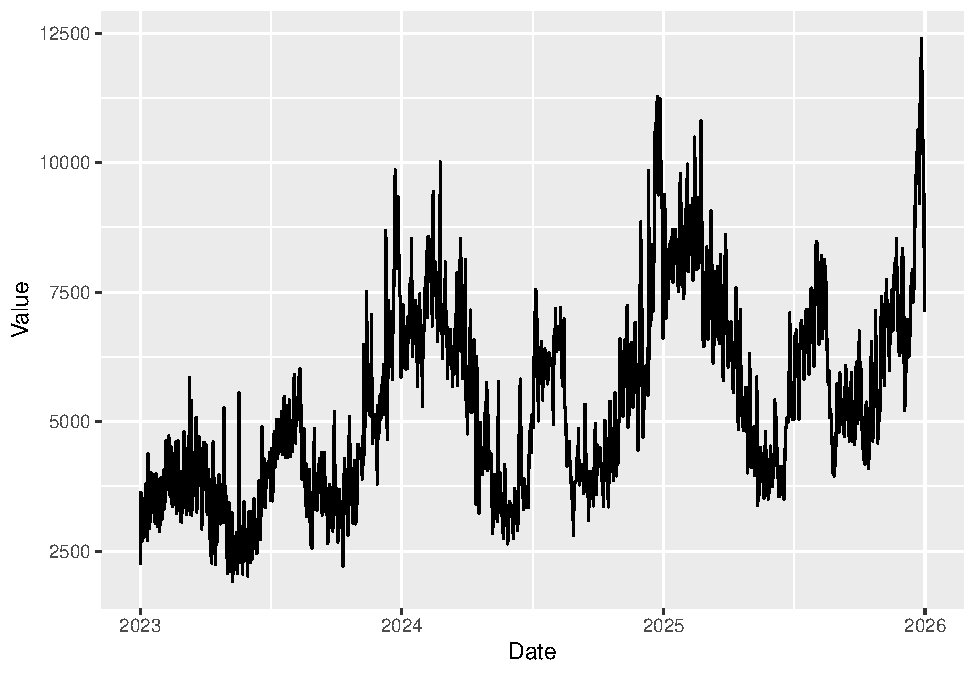
\includegraphics[keepaspectratio]{paper_files/paper_files/figure-latex/unnamed-chunk-1-1.pdf}}

\begin{Shaded}
\begin{Highlighting}[]
\FunctionTok{ggplot}\NormalTok{(ts,}
  \FunctionTok{aes}\NormalTok{(}
    \AttributeTok{x =}\NormalTok{ Date,}
    \AttributeTok{y =}\NormalTok{ Value,}
   \AttributeTok{fill =}\NormalTok{ Value}
\NormalTok{  ) ) }\SpecialCharTok{+}
  \FunctionTok{geom\_tsspiral}\NormalTok{(}
    \AttributeTok{ring\_spacing =} \DecValTok{2}
\NormalTok{   ) }\SpecialCharTok{+}
   \FunctionTok{scale\_fill\_viridis\_c}\NormalTok{() }\SpecialCharTok{+}
   \FunctionTok{theme\_void}\NormalTok{()}
\end{Highlighting}
\end{Shaded}

\pandocbounded{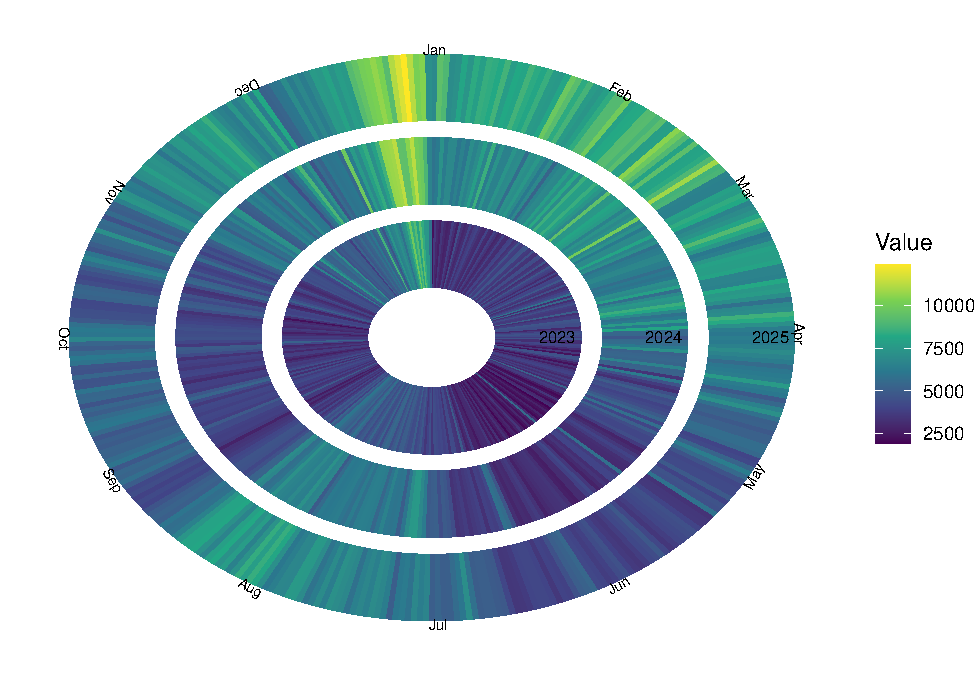
\includegraphics[keepaspectratio]{paper_files/paper_files/figure-latex/unnamed-chunk-2-1.pdf}}

\section{State of the field}\label{state-of-the-field}

``Spiral layout has two major advantages for data visualization. First,
it is able to visualize data with long axes, which greatly improves the
resolution of visualization. Second, it is efficient for time series
data to reveal periodic patterns''

The R package \texttt{spiralize}(Gu \& Huebschmann, 2021) provides tools
for visualising time series data using spiral layouts. Building on this
idea, our package introduces a new set of geoms that integrate with
ggplot2, extending the grammar of graphics to spiral-based
visualisation. This integration allows users to construct spiral plots
using a familiar and flexible syntax while retaining the layered
approach to data visualisation that makes ggplot2 powerful. Rather than
treating spiral plots as standalone graphics, our approach brings them
into the grammar of graphics framework, enabling users to explore
temporal patterns through a broader range of visual encodings. The R
package \texttt{spiralize} provides tools for visualising data using
spiral layouts. In our approach, we introduce a circular representation
of time series data, which we define as a spiral: our approach
represents time series data using circular layouts, arranging
observations around circles to highlight periodicity, seasonality, and
recurring temporal patterns.

What has been missing is a reusable tool for creating spiral
visualisations of time series data that supports the exploration of
temporal patterns across multiple time scales. Compared with
conventional time series plotting tools, \texttt{tsspiral} adds:

\begin{itemize}
\tightlist
\item
  Spiral visualisations of time series using polar coordinates.
\item
  Alternative representations of temporal patterns, making recurring
  cycles and seasonal variations easier to explore.
\item
  A framework for visualising temporal hierarchies, from annual and
  quarterly patterns to monthly, weekly, and daily observations.
\item
  New
\item
  An open-source implementation in R that supports reproducible
  visualisation workflows.
\item
  A flexible approach that can be incorporated into statistical
  analysis, research communication, and teaching.
\end{itemize}

Rakuschek et al. (2026) pointed out circular version of time series
plots has both advantage and disadvantages. Hence Rakuschek et al.
(2026) suggested to use both line and circular version of the plots to
get a better idea of the data rather than using circular plots as a
replacement to line plots.

\section{Software design}\label{software-design}

Each circle is split in to 365. For a leap year circle is divided in to
,,segments. When visualising quarterly data all dates corresponds to
that is colour.

\texttt{tsspiral} introduces a new set of \texttt{ggplot2} geoms that
integrate seamlessly with the \texttt{ggplot2} grammar of graphics to
create spiral time series plots. This design allows users to generate
spiral visualisations within familiar R plotting workflows while
retaining the flexibility and composability of \texttt{ggplot2}.

\begin{Shaded}
\begin{Highlighting}[]
\FunctionTok{library}\NormalTok{(patchwork)}
\FunctionTok{library}\NormalTok{(tsspiral)}
\NormalTok{p1 }\OtherTok{\textless{}{-}} \FunctionTok{ggplot}\NormalTok{(beans\_dambulla, }\FunctionTok{aes}\NormalTok{(}\AttributeTok{x=}\NormalTok{Date, }\AttributeTok{y=}\NormalTok{Price, }\AttributeTok{fill=}\NormalTok{Price)) }\SpecialCharTok{+} \FunctionTok{geom\_tsspiral}\NormalTok{() }\SpecialCharTok{+} \FunctionTok{ggtitle}\NormalTok{(}\StringTok{"A"}\NormalTok{)}
\NormalTok{p2 }\OtherTok{\textless{}{-}} \FunctionTok{ggplot}\NormalTok{(beans\_dambulla, }\FunctionTok{aes}\NormalTok{(}\AttributeTok{x=}\NormalTok{Date, }\AttributeTok{y=}\NormalTok{Price, }\AttributeTok{fill=}\NormalTok{Price)) }\SpecialCharTok{+} \FunctionTok{geom\_tsspiralbar}\NormalTok{() }\SpecialCharTok{+} \FunctionTok{ggtitle}\NormalTok{(}\StringTok{"B"}\NormalTok{)}
\NormalTok{p3 }\OtherTok{\textless{}{-}} \FunctionTok{ggplot}\NormalTok{(beans\_dambulla, }\FunctionTok{aes}\NormalTok{(}\AttributeTok{x=}\NormalTok{Date, }\AttributeTok{y=}\NormalTok{Price, }\AttributeTok{fill=}\NormalTok{Price)) }\SpecialCharTok{+} \FunctionTok{geom\_tsspiralmiss}\NormalTok{() }\SpecialCharTok{+} \FunctionTok{ggtitle}\NormalTok{(}\StringTok{"C"}\NormalTok{)}
\NormalTok{p4 }\OtherTok{\textless{}{-}} \FunctionTok{temporal\_hierarchical}\NormalTok{(}
 \AttributeTok{data =}\NormalTok{ beans\_dambulla,}
 \AttributeTok{date =}\NormalTok{ Date,}
 \AttributeTok{value =}\NormalTok{ Price)}
\NormalTok{(p1}\SpecialCharTok{|}\NormalTok{p2)}\SpecialCharTok{/}\NormalTok{(p3}\SpecialCharTok{|}\NormalTok{p4)}
\end{Highlighting}
\end{Shaded}

\section{Research impact statement}\label{research-impact-statement}

tsspiral expands the ways researchers can explore time series through a
circular shape. By representing time series on a polar coordinates, the
package provides alternative way to explore temporal patterns, recurring
cycles and changes over time. furthermore, this allows to visualise
temporal-hierarchcical time series. By aggregating time series under
different temporal scales from years to quarters, months, weeks, and
days, spiral visualisations can reveal recurring seasonal patterns and
relationships between different temporal scales. This allows researchers
to explore patterns in the time series within and across years,
quarters, months, or other time intervals.

\section{AI usage disclosure}\label{ai-usage-disclosure}

ChatGPt was used to assist with code development and documentation
roxygen files writing.

\section*{References}\label{references}
\addcontentsline{toc}{section}{References}

\phantomsection\label{refs}
\begin{CSLReferences}{1}{0}
\bibitem[\citeproctext]{ref-spiralize}
Gu, Z., \& Huebschmann, D. (2021). Spiralize: An r package for
visualizing data on spirals. \emph{Bioinformatics}.
doi:\href{https://doi.org/10.1093/bioinformatics/btab778}{10.1093/bioinformatics/btab778}

\bibitem[\citeproctext]{ref-rakuschek2026guided}
Rakuschek, J., Hauser, H., \& Schreck, T. (2026). Guided spiral
visualization for periodic time series and residual analysis.
\emph{Computers \& Graphics}, 104535.

\bibitem[\citeproctext]{ref-tukey1977exploratory}
Tukey, J. W. et al. (1977). \emph{Exploratory data analysis} (Vol. 2).
Addison-wesley, Reading, MA.

\bibitem[\citeproctext]{ref-weber2001visualizing}
Weber, M., Alexa, M., \& Müller, W. (2001). Visualizing time-series on
spirals. \emph{Infovis} (Vol. 1, pp. 7--14).

\end{CSLReferences}

\end{document}
